\documentclass[11pt]{article}
\usepackage[T1]{fontenc}

% Set page size and margins
% Replace `letterpaper' with`a4paper' for UK/EU standard size
\usepackage[a4paper,top=2cm,bottom=2cm,left=3cm,right=3cm,marginparwidth=1.75cm]{geometry}

% Useful packages
\usepackage{amsmath}
\usepackage{graphicx}
\usepackage{amsfonts}
\usepackage{fancyhdr}
\setlength{\headheight}{15pt}
\pagestyle{fancy}

\usepackage{hyperref}
\hypersetup{
    colorlinks,
    citecolor=black,
    filecolor=black,
    linkcolor=black,
    urlcolor=black
}

\usepackage{glossaries}
\usepackage{subfigure}

\makenoidxglossaries


\loadglsentries{lexique}


\usepackage{xcolor}

\usepackage{eso-pic}
\usepackage{tikz}
\usetikzlibrary{shapes,arrows,positioning}
\usepackage{float}
\usepackage{textcomp}
\usepackage{soul}
\usepackage{listings}
\newcommand{\hilight}{\makebox[0pt][s]{\color{green!50}\rule[-3.6pt]{1.0\linewidth}{12pt}}}

\usepackage{tikz}

\definecolor{mygray}{rgb}{0.5,0.5,0.5}
\lstdefinestyle{command}{
  backgroundcolor=\color{white},
  basicstyle=\ttfamily\color{black},
  keywordstyle=\color{blue},
  commentstyle=\color{mygray},
  stringstyle=\color{red},
  showstringspaces=false,
  upquote=true,
  morekeywords={sudo, ls, cd, mv, cp, rm, mkdir, chmod, chown, grep, find},
  captionpos=b,
  frame=single,
  numbers=left,
  numberstyle=\tiny\color{mygray},
  breaklines=true,
  breakatwhitespace=true,
  tabsize=2,
  keepspaces=true,
  caption={Linux Command},
  label=command,
}
\lstdefinestyle{bashstyle}{
  backgroundcolor=\color{white},
  basicstyle=\ttfamily\color{black},
  keywordstyle=\color{blue},
  commentstyle=\color{mygray},
  stringstyle=\color{red},
  showstringspaces=false,
  upquote=true,
  morekeywords={sudo, ls, cd, mv, cp, rm, mkdir, chmod, chown, grep, find},
  captionpos=b,
  frame=single,
  numbers=left,
  numberstyle=\tiny\color{mygray},
  breaklines=true,
  breakatwhitespace=true,
  tabsize=2,
  keepspaces=true,
  caption={Script bash},
  label=command,
}

\lstdefinestyle{cstyle}{
    language=C,
    basicstyle=\ttfamily,
    keywordstyle=\color{blue},
    commentstyle=\color{green!40!black},
    stringstyle=\color{red},
    identifierstyle=\color{black},
    captionpos=b,
    numbers=left,
    numberstyle=\tiny\color{gray},
    frame=single,
    breaklines=true,
    showstringspaces=false,
    tabsize=4,
    morekeywords={int, char, void, if, else, while, for, return, typedef, struct, include},
    columns=flexible
}

\lstdefinestyle{makefilestyle}{
    language=make,
    basicstyle=\ttfamily,
    keywordstyle=\color{blue},
    commentstyle=\color{green!40!black},
    captionpos=b,
    stringstyle=\color{red},
    identifierstyle=\color{black},
    numbers=left,
    numberstyle=\tiny\color{gray},
    frame=single,
    breaklines=true,
    showstringspaces=false,
    tabsize=4,
    morekeywords={ifeq, endif, else, ifdef, ifndef, define, endef, export, unexport, obj},
    columns=flexible
}
\lstdefinestyle{config}{
    language=make,
    basicstyle=\ttfamily,
    keywordstyle=\color{blue},
    commentstyle=\color{green!40!black},
    captionpos=b,
    stringstyle=\color{red},
    identifierstyle=\color{black},
    numbers=left,
    numberstyle=\tiny\color{gray},
    frame=single,
    breaklines=true,
    showstringspaces=false,
    tabsize=4,
    morekeywords={ifeq, endif, else, ifdef, ifndef, define, endef, export, unexport, obj},
    columns=flexible
}

\bibliographystyle{plain} % We choose the "plain" reference style

\renewcommand{\epsilon}{\varepsilon} 
\renewcommand{\phi}{\varphi} 
\title{Final year project report\vspace{10pt}\\**************************************************\\Multi agent scene exploration and mapping \\
for civil engineering progress tracking\vspace{10pt} \\**************************************************}
\author{BELPOIS Vincent \\ Under the supervision of Dr. Ivan \textsc{Mutis}}

\begin{document}

\date{2024}
\maketitle
\thispagestyle{empty}

\vspace{10mm}

    \begin{center}
    
\includegraphics[width = 6cm]{Images/logo_ensma.png}
    \end{center}
    \vspace{2cm}
    \begin{center}
        
\includegraphics[width = 8cm]{Images/IIT_Logo_stack_186_blk.png}
    \end{center}
    \newpage
    \thispagestyle{empty}
    \mbox{}
    
    

    
    \AddToShipoutPictureBG{%
    \put(15,7){
\includegraphics[scale = 0.02]{Images/logo_ensma.png}}
    \put(480,10){
\includegraphics[width = 100pt]{Images/IIT_Logo_stack_186_blk.png}}
    
    }



    \newpage
    \section*{Acknowledgments}

        Acknowledgments.
        
    \newpage
    \thispagestyle{empty}
    \mbox{}
    \newpage
    \thispagestyle{empty}
    {\small \tableofcontents}

    \newpage
    \thispagestyle{empty}
    \mbox{}
    \newpage
    
    \section{Introduction}
    
        Introduction    

        $$
        \int_\alpha^\beta f(x) dx
        $$
        \cite{xu2022fast}


    \newpage
    
    \section[Setting up the physical agents]{Setting up the physical agents}
    \label{section:big title}%label to reference section

        Three platforms were used in this project, a six wheeled platform, a quadcopter and a quadruped platform. Each platform was chosen for its specific characteristics and the goal was to have a multi agent system that could explore a scene and map it. The six wheeled platform was chosen for its stability and its ability to carry heavy loads. The quadcopter was chosen for its ability to fly and to have a bird's eye view of the scene. The quadruped platform was chosen for its ability to climb stairs and to have a low center of gravity.

    
        \subsection{Six wheeled platform setup}

            The six wheeled platform was chosen for its stability and its ability to carry heavy loads, the intent was to have it carrying a robotic arm for other projects.
            Some previous work was already done on the platform but were apparently unsuccessful. These earlier attempts had left the platform in a partially modified state, requiring a comprehensive reassessment and redesign of both the mechanical and electrical systems. Despite these setbacks, the robust chassis of the six-wheeled platform still presented an excellent foundation for our project, offering the potential for a versatile and capable vehicle once properly configured.

            \subsubsection{Mechanical modifications}
            As it arrived, the six wheeled platform only consisted of a stainless steel chassis and 6 DC motors and wheels. The platform required several mechanical modifications to accommodate the necessary components for autonomous operation. Specifically, it needed a mount for a Lidar sensor and an embedded computer on its top surface \ref{fig:lidar_mount}. Additionally, a mounting solution for the motor drivers on the inside of the chassis was essential \ref{fig:motor_driver_mount}. These modifications were designed and implemented to ensure proper integration of all components while maintaining the structural integrity of the platform \ref{fig:full_cad_model}.

            \begin{figure}[htbp]
                \centering
                LIDAR MOUNT CAD
                %\includegraphics[width=0.8\textwidth]{images/lidar_mount_cad.png}
                \caption{CAD model of the Lidar sensor and embedded computer mount}
                \label{fig:lidar_mount}
            \end{figure}
            
            \begin{figure}[htbp]
                \centering
                MOTOR DRIVER MOUNT CAD
                %\includegraphics[width=0.8\textwidth]{images/motor_driver_mount_cad.png}
                \caption{CAD model of the motor driver mounting solution}
                \label{fig:motor_driver_mount}
            \end{figure}
            
            \begin{figure}[htbp]
                \centering
                FULL PLATFORM CAD
                %\includegraphics[width=0.8\textwidth]{images/full_platform_cad.png}
                \caption{Full CAD model of the modified six-wheeled platform}
                \label{fig:full_cad_model}
            \end{figure}

            \subsubsection{Electronics architecture}
                The essential electronic components needed to get the platform running were mainly DC motor drivers to drive the motors, a Lidar sensor and an embedded computer.
                
                Difficulties were encountered when trying to use the drivers someone else tried before hand as they were underpowered : at stall, the motors required around 5 amps, as measured with a bench top power supply, and the drivers I was trying to use were only capable of delivering 2 amps per channel or a total of 4 amps when combining outputs. The drivers in question were the \color{red} INSERT REFERENCE \color{black} which were in terms replaced by the driver \color{red} INSERT REFERENCE \color{black}. A physical comparison can be seen in \ref{fig:drivers_compraison}
                
                Difficulties were encountered when trying to use the drivers someone else tried before hand as they were underpowered : at stall, the motors required around 5 amps, as measured with a bench top power supply, and the drivers I was trying to use were only capable of delivering 2 amps per channel or a total of 4 amps when combining outputs. The drivers in question were the L298N H-bridge motor drivers, which were ultimately replaced by the DFRobot 7A Dual DC Motor Driver. The L298N drivers, while popular for smaller projects, proved inadequate for the power requirements of our six-wheeled platform. In contrast, the DFRobot 7A Dual DC Motor Driver offer a continuous current output of 7A per channel, more than sufficient for our needs. This upgrade significantly improved the platform's performance, allowing for smoother operation and better handling of the motor's power demands. A physical comparison of these drivers can be seen in Figure.\ref{fig:drivers_comparison}.

                
                \begin{figure}[h]
                    \centering
                    INSERT (a) (b) PICTURE OF BOTH DRIVERS
                    \caption{Comparison of L298N (a) and DFRobot 7A dial DC Motor Driver (b)}
                    \label{fig:drivers_comparison}
                \end{figure}

                The three motor drivers were connected to microcontroller. The connection can be seen in \ref{fig:driver_to_pico}.
                I chose to use a Raspberry pi Pico microcontroller for it's many outputs at a total of \color{red} XX general purpose input outputs (GPIO) \color{black}. Each driver required 6 control signals or 3 per motor : Two signals are used to control the direction of the motor according to table \color{red} MAKE AND CITE TABLE DIR \color{black} while the third signal's duty cycle determine the speed.

                A radio control (RC) receiver was also connected to interrupt capable GPIOs of the microcontroller to be able to control the platform manually. Three channels of the RC receiver were used to control the speed, the direction and the mode of the platform. The mode refers to whether or not the platform is in manual control or in autonomous mode and is connected to channel 5 of the radio which has a two way switch.

                Finally, the pico is connected to an Nvidia Jetson Orin single board computer (SBC) via USB. This connection is used both to reprogram the pico, as well as to send speed and direction commands to each motor via a serial communication. 

                Not including the power distribution and regulation system, \ref{fig:overall_electical_system} shows the electrical connections of these components on the modified six-wheeled platform.

                \begin{figure}[h]
                    \centering
                    OVERALL ELECTRICAL SYSTEM (excluding power)
                    \label{fig:overall_electical_system}
                \end{figure}


                
                
                \begin{figure}[h]
                    \centering
                    Driver to PICO connection diagram
                    \label{fig:driver_to_pico}
                \end{figure}

            
            
            \subsubsection{Software architecture}

            How the software on the jetson communicates with the microcontroller and how it communicates with the lidar. The choice of the odometry algorithm will be explain in another section (master, comparison of multiple algo)

            The robot operation system (ROS) was chosen as the software framework for the platform running on the Jetson Orin embedded computer. Specifically, ROS2 Humble Hawksbill was selected due to its extensive package availability and compatibility with the Jetson Orin's hardware. Indeed, as I as made aware of the strugles of someone else running a ROS based robot on an Nvidia Jetson Nano and how Ubuntu, and ROS version mismatch may bring problems. 
            
            This version of ROS2 provides a robust and flexible framework for developing and integrating various components of the platform, including sensor processing, navigation, and control. For real-time critical tasks such as motor control and RC radio interrupts, the Raspberry Pi Pico microcontroller was utilized, leveraging its ability to handle low-level, time-sensitive operations. The microcontroller's firmware was developed from the ground up by myself, guaranteeing reliable execution of motor control and interrupt handling tasks. By combining the strengths of ROS2 on the Jetson Orin with the real-time capabilities of the Raspberry Pi Pico, the platform achieves a robust and efficient software architecture that enables seamless integration of autonomous navigation, sensor processing, and manual control.

            %! Add a reference to this figure !!
            \begin{figure}[H]
                \centering
                %Software stack, from jetpack to ros2 to the nodes to the microcontroller
                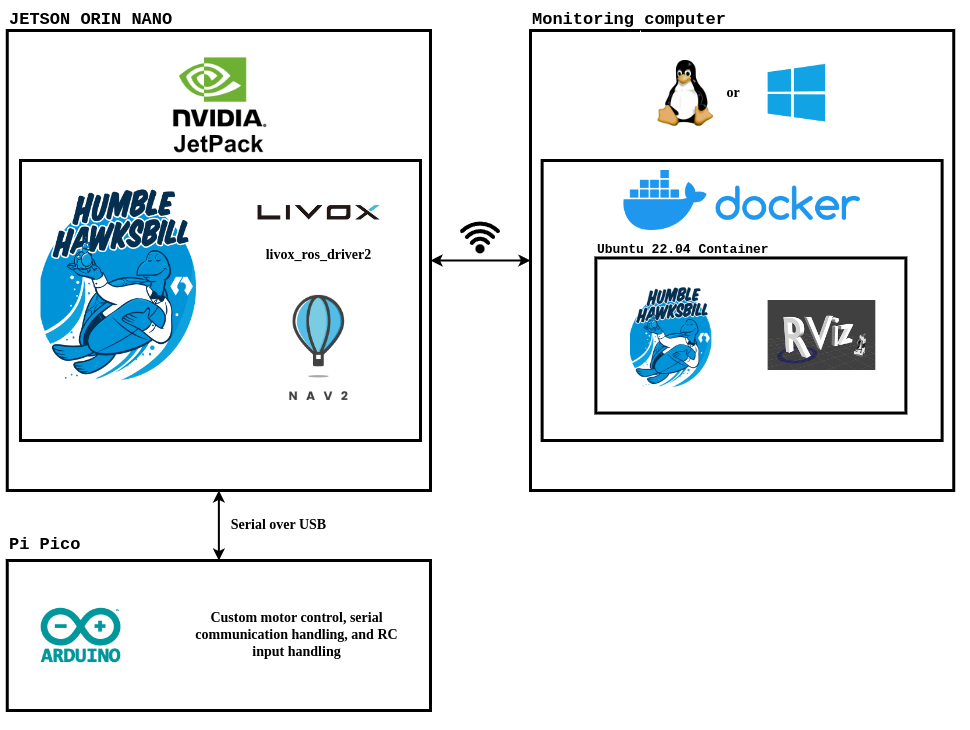
\includegraphics[width=0.8\textwidth]{Images/Software architecture rover.drawio.png}
                \caption{Software architecture}
                \label{fig:SW_architecture}
            \end{figure}


            \subsubsection{ROS 2 setup}
            
            %What nodes did I create, explain the setup with nav2 working.


            \subsubsection{Issues encountered}
                
            Explain the state reached (nav2 navigation kinda working) and why the other platform was created

            \begin{figure}[H]
                \centering 
                \subfigure[Version 1 of the rover]{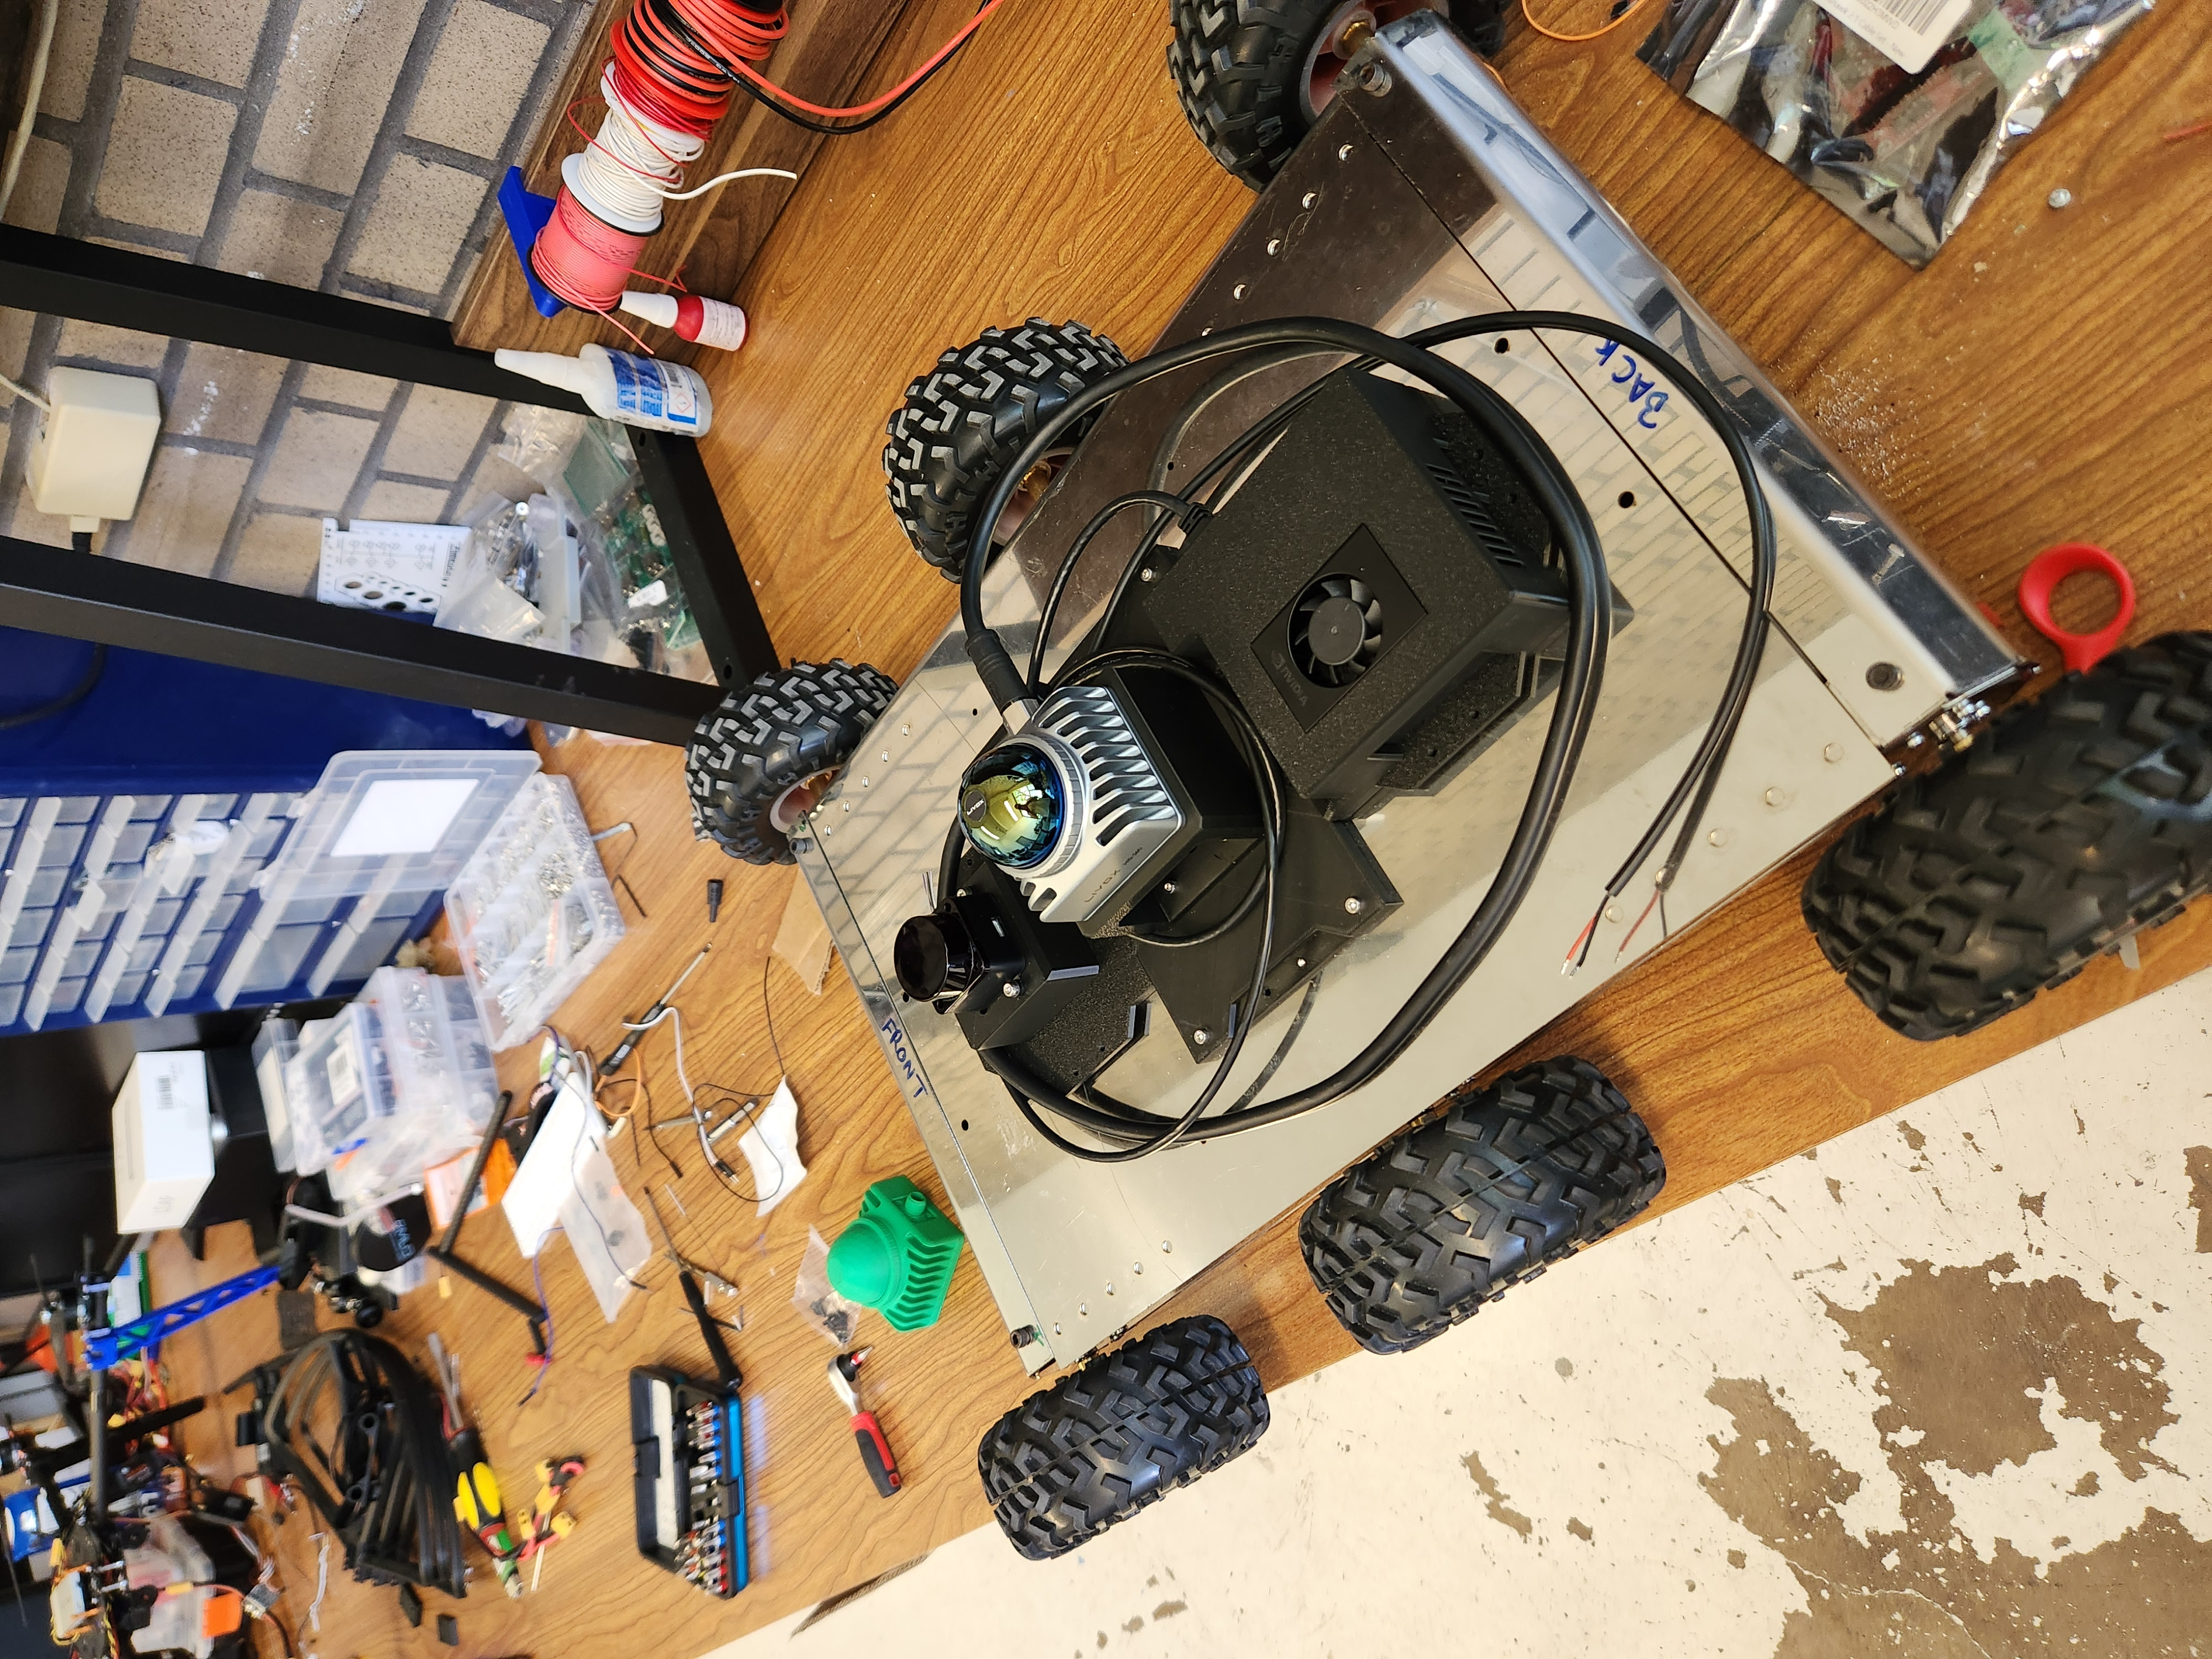
\includegraphics[width=0.4\textwidth, angle=270]{Images/roverv1closed.jpg}}
                \subfigure[Version 2 of the rover]{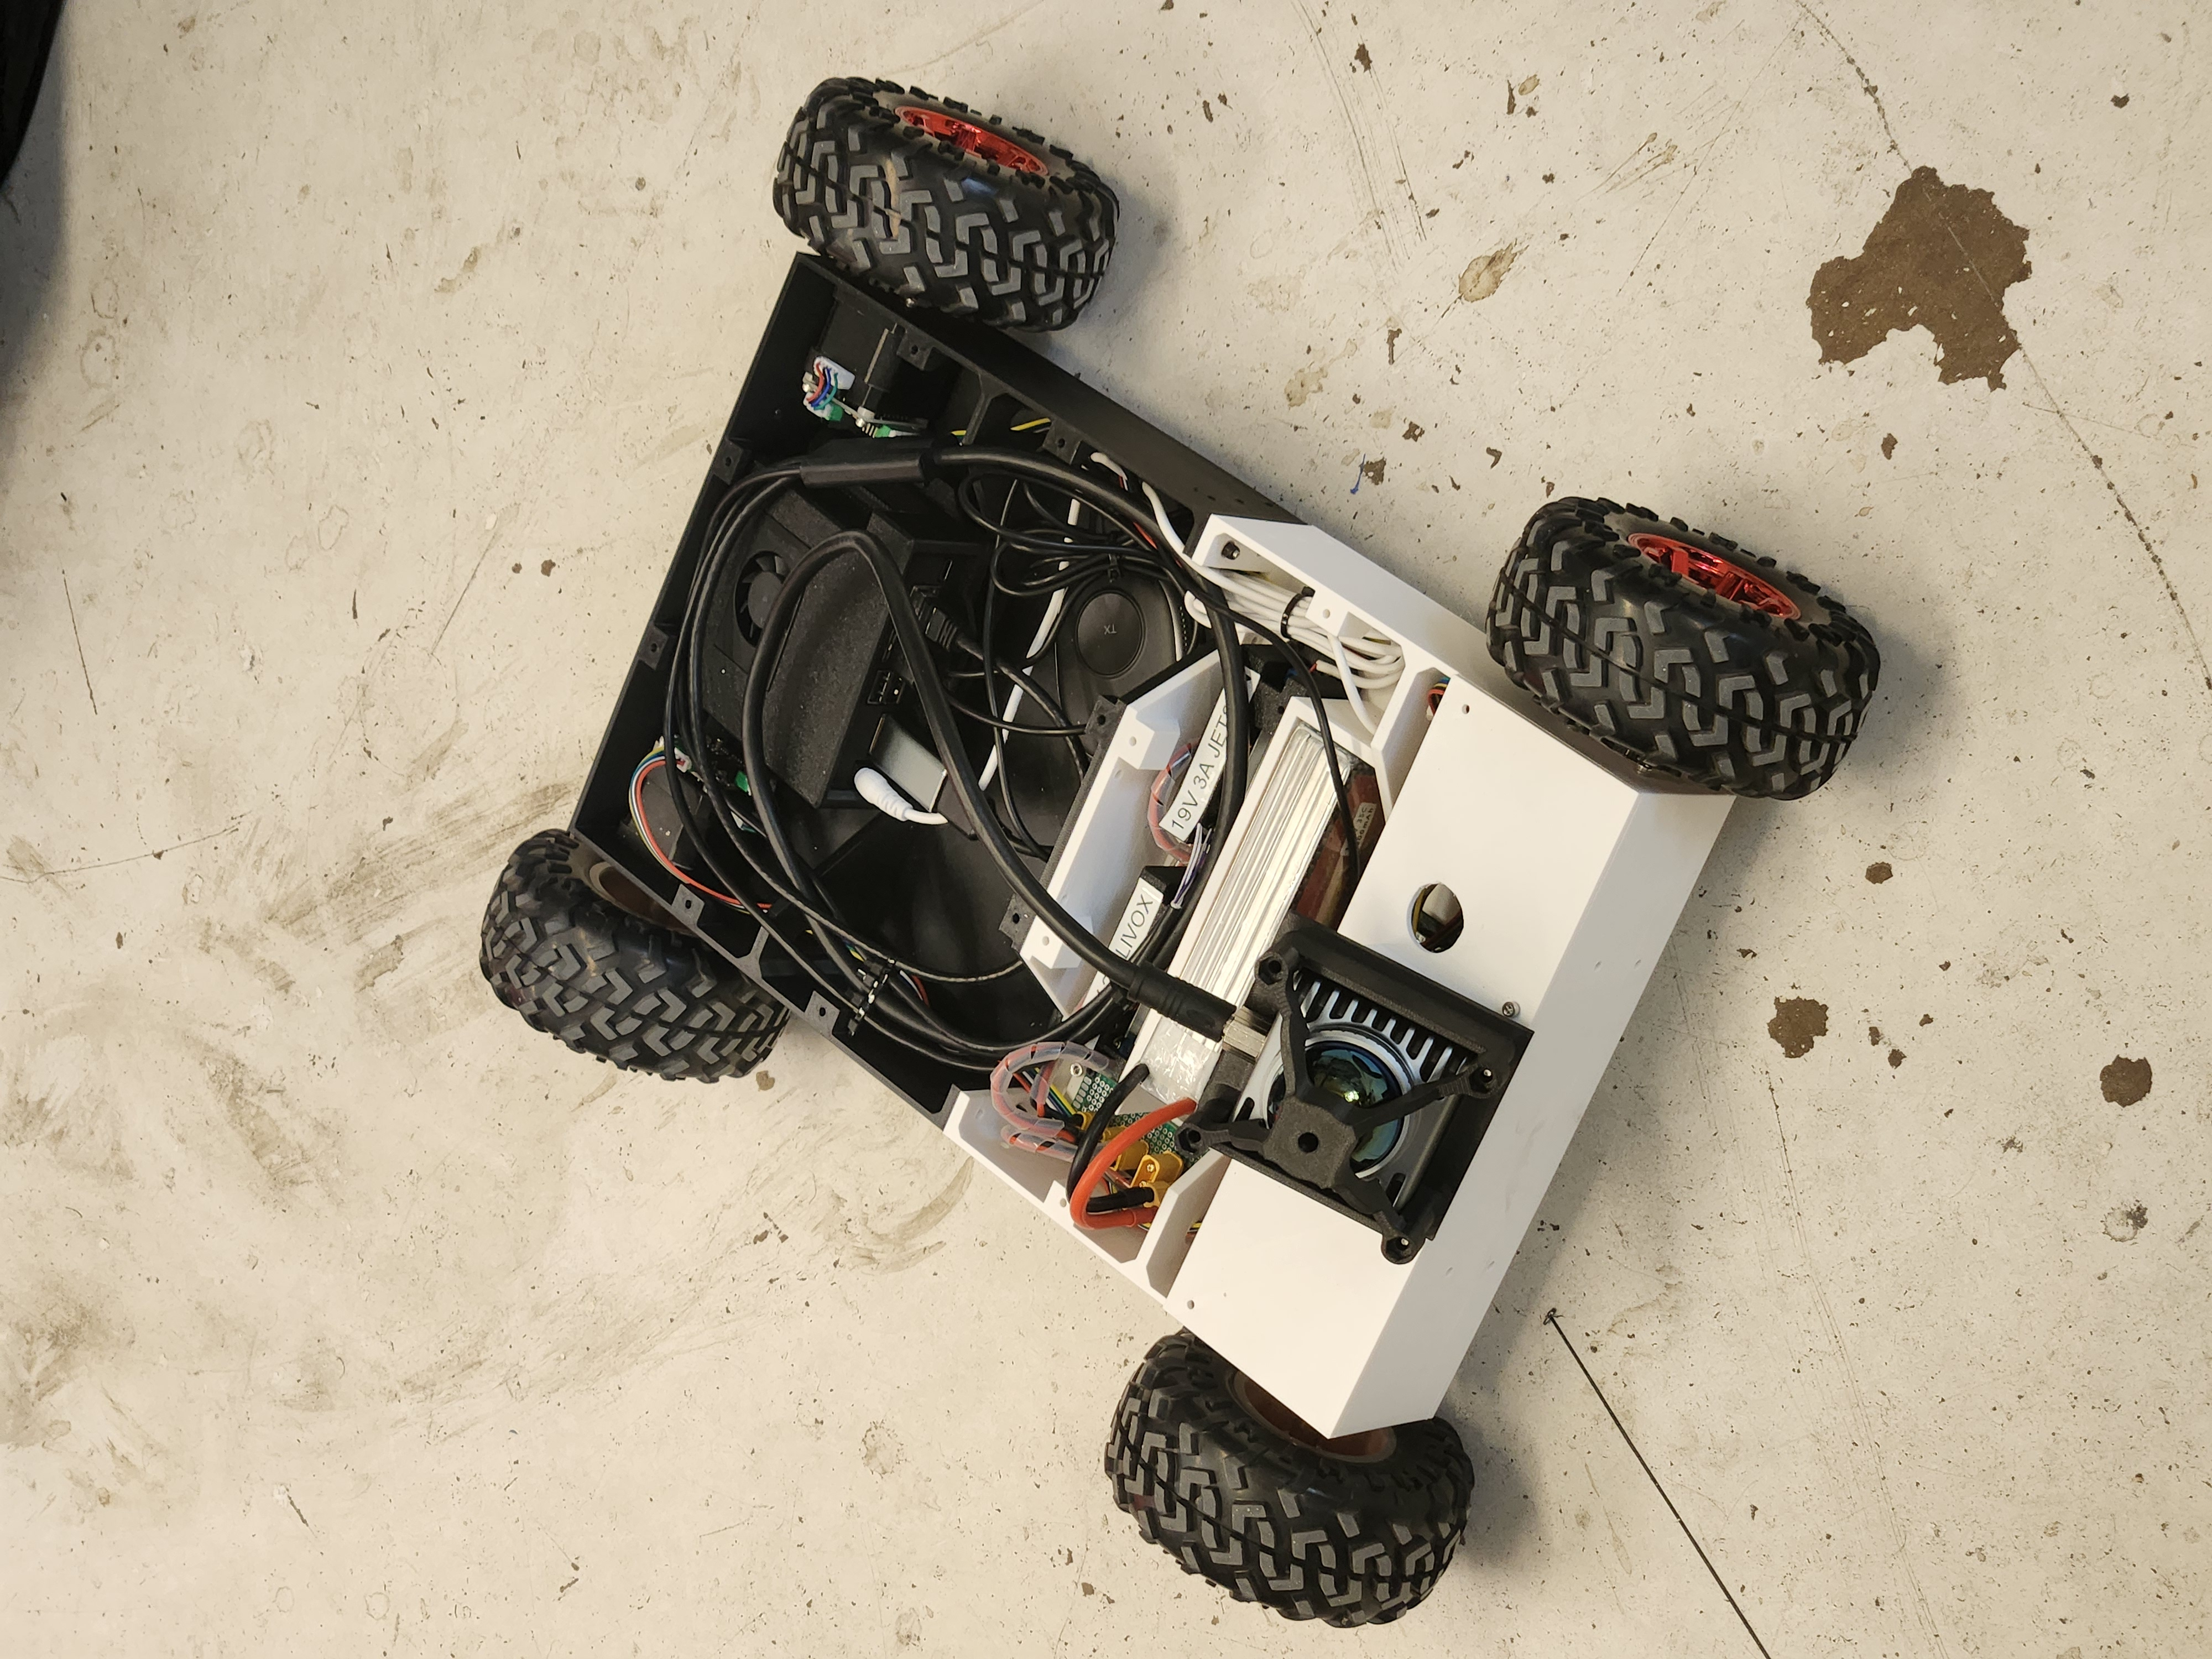
\includegraphics[width=0.4\textwidth, angle=270]{Images/roverv2openened.jpg}}       
            \end{figure}


            Explain how the chassis was designed to fit the new closed loop, motors
`
        \subsection{Quadcopter setup}
                
                % Explain the platform's starting point and the goal
                % Explain the different drones that were at my disposal and which one was selected for our application (the one that could easel;y carry the lidar, jetson while not being too big)

                One of the agents in our multi-agent system is a quadcopter, chosen for its ability to provide aerial perspective and navigate in three-dimensional space. After evaluating several drone options available to us, we selected a model that struck an optimal balance between payload capacity and size. This drone was capable of easily carrying the Livox Mid-360 Lidar sensor and the Nvidia Jetson Orin embedded computer, while still maintaining a compact form factor suitable for indoor and outdoor operations.

                The quadcopter platform required several modifications to integrate our specific sensor suite and computational hardware.

                \subsubsection{Mechanical modifications}

                    I designed and 3D printed new landing legs that fit on the arms of the quadcopter. Those landing legs were designed to increase the landing stability, which I noticed was a problem in the manual flight I performed, and to reduce the blindspots of the lidar which was to be placed on the center of the underside of the drone.

                    I also took the oportunity to redisgne the battery mounting mechanism which was hbulky, heavy, and suitable to only one size of battery to one that is much simpler and uses velcro straps as can been seen in Figure \ref{fig:landing_legs}.
                    

                    \begin{figure}[H]
                        \centering
                        FIGURES OF BOTH THE LANDING LEGS 3D MODEL, THE OLD BATTERY TRAY AND THE NEW ONE.
                        \caption{Landing legs and battery tray}
                        \label{fig:landing_legs}
                    \end{figure}    
                \subsubsection{Electronics architecture}
    
                    % Similarly to the rover, the jetson is still connected to the LIDAR via ethernet 
                    % The drone is controlled by a PLACEHOLDER_CONTROLLER, which is connected to the jetson via USB

                    To keep the architecture similar to the one used on the wheeled robot, 

                \subsubsection{Software architecture and setup}
    
            
                \subsubsection{Issues encountered}
                
        \subsection{Quadruped platform setup}


            \subsubsection{Mechanical modifications}

            How the top part was scanned to be replaced for a jetson, and a lidar to be mounted

            \subsubsection{Compute backpack}

            Explain how the jetson, the lidar and the robot communicate.

            As is the case with the wheeled platform and the drone, we chose to use a Livox Mid-360 lidar and a Nvidia Jetson Orin embedded computer. Even though the quadruped already carries a 3D Lidar, we chose to use a Mid-360 to have a more accurate 3D map and to standardize the platforms.


            \begin{figure}[H]
                \centering
                IMAGE OF COMPUTE BACKPACK
            \end{figure}


            \begin{figure}[H]
                \centering
                IMAGE OF SCANNER AND SCANNED TOP OF ROBOT
            \end{figure}

            \subsubsection{Issues encountered}

            Big battery issue, reverse engineering of the battery


            \begin{figure}[H]
                \centering
                IMAGE OF DISASEMBLED BATTERY
            \end{figure}

        \newpage

    \section{Mapping, planning, and exploration algorithms}

        \subsection{Mapping}
            \subsubsection{Introduction to SLAM}
            \subsubsection{Comparison of odometry algorithms}

        \subsection{Planning}
            \subsubsection{Path planning}
            \subsubsection{2D path planning}
            \subsubsection{Comparison of 3D planning algorithms}

        \subsection{Exploration}
            \subsubsection{Metrics for exploration}
            \subsubsection{TARE-PLANNER}
            \subsubsection{MTARE-PLANNER}
            \subsubsection{Comparison of exploration algorithms}

    \newpage
    \section{Simulation}
        \subsection{Choosing a simulation environment}

            To test the algorithms and the coordination of the different platforms, a simulation environment was needed. The choice of the simulation environment was based on the following criteria : being able to simulate multiple platforms, being able to simulate the sensors we had on the physical platforms, and the portability of the simulation environment.


            \subsubsection{Gazebo}
                Gazebo is a well known simulation environment in the robotics community. It is widely used and has a large community. It is open source and has a lot of plugins available, for simulation sensors, motion platforms and more. As I was already familiar with it, I first looked at it to build a crude simulation of the 6 wheeled platform. Thanks to the use of ROS2 and ROS2-control for the drive train, I was able to quickly build a simulation of the platform. 

                I was also able to find a working simulation of the Livox Mid-360 Lidar sensor we chose for every platform. The package \cite{livox_lidar_simulation_fork} was a fork of the original simulation package from Livox \cite{livox_laser_simulation} and was modified to work with the specific lidar we are using. 
            \subsubsection{Nvidia Isaac Sim}

                Isaac sim is a high fidelity simulation environment developed by Nvidia. This simulation environment uses a PhysX based physics engine and is able to simulate multiple platforms at once. It is also able to simulate sensors like cameras, lidars and IMUs. The main advantage of Isaac sim is it's high fidelity and parallelization. However, this also brings a lot of complexity and the need for a RTX GPU to run it.

                The high overhead, complexity, low portability and the fact that it was not open source made me choose Gazebo over Isaac sim for the simulation of the platforms.

                In addition, the Lidar we are using has a non repetitive pattern, which is not currently supported by Isaac sim and would have required a lot of work to simulate.

                I did experiment with Isaac sim to simulate the quadruped platform, as it was the most complex platform to simulate and there existed a simulation of the robot in Isaac sim.
        \subsection{Simulating sensors}
            \subsubsection{Lidar}

            \begin{figure}[H]
                \centering
                \subfigure[Gazebo simulation environment]{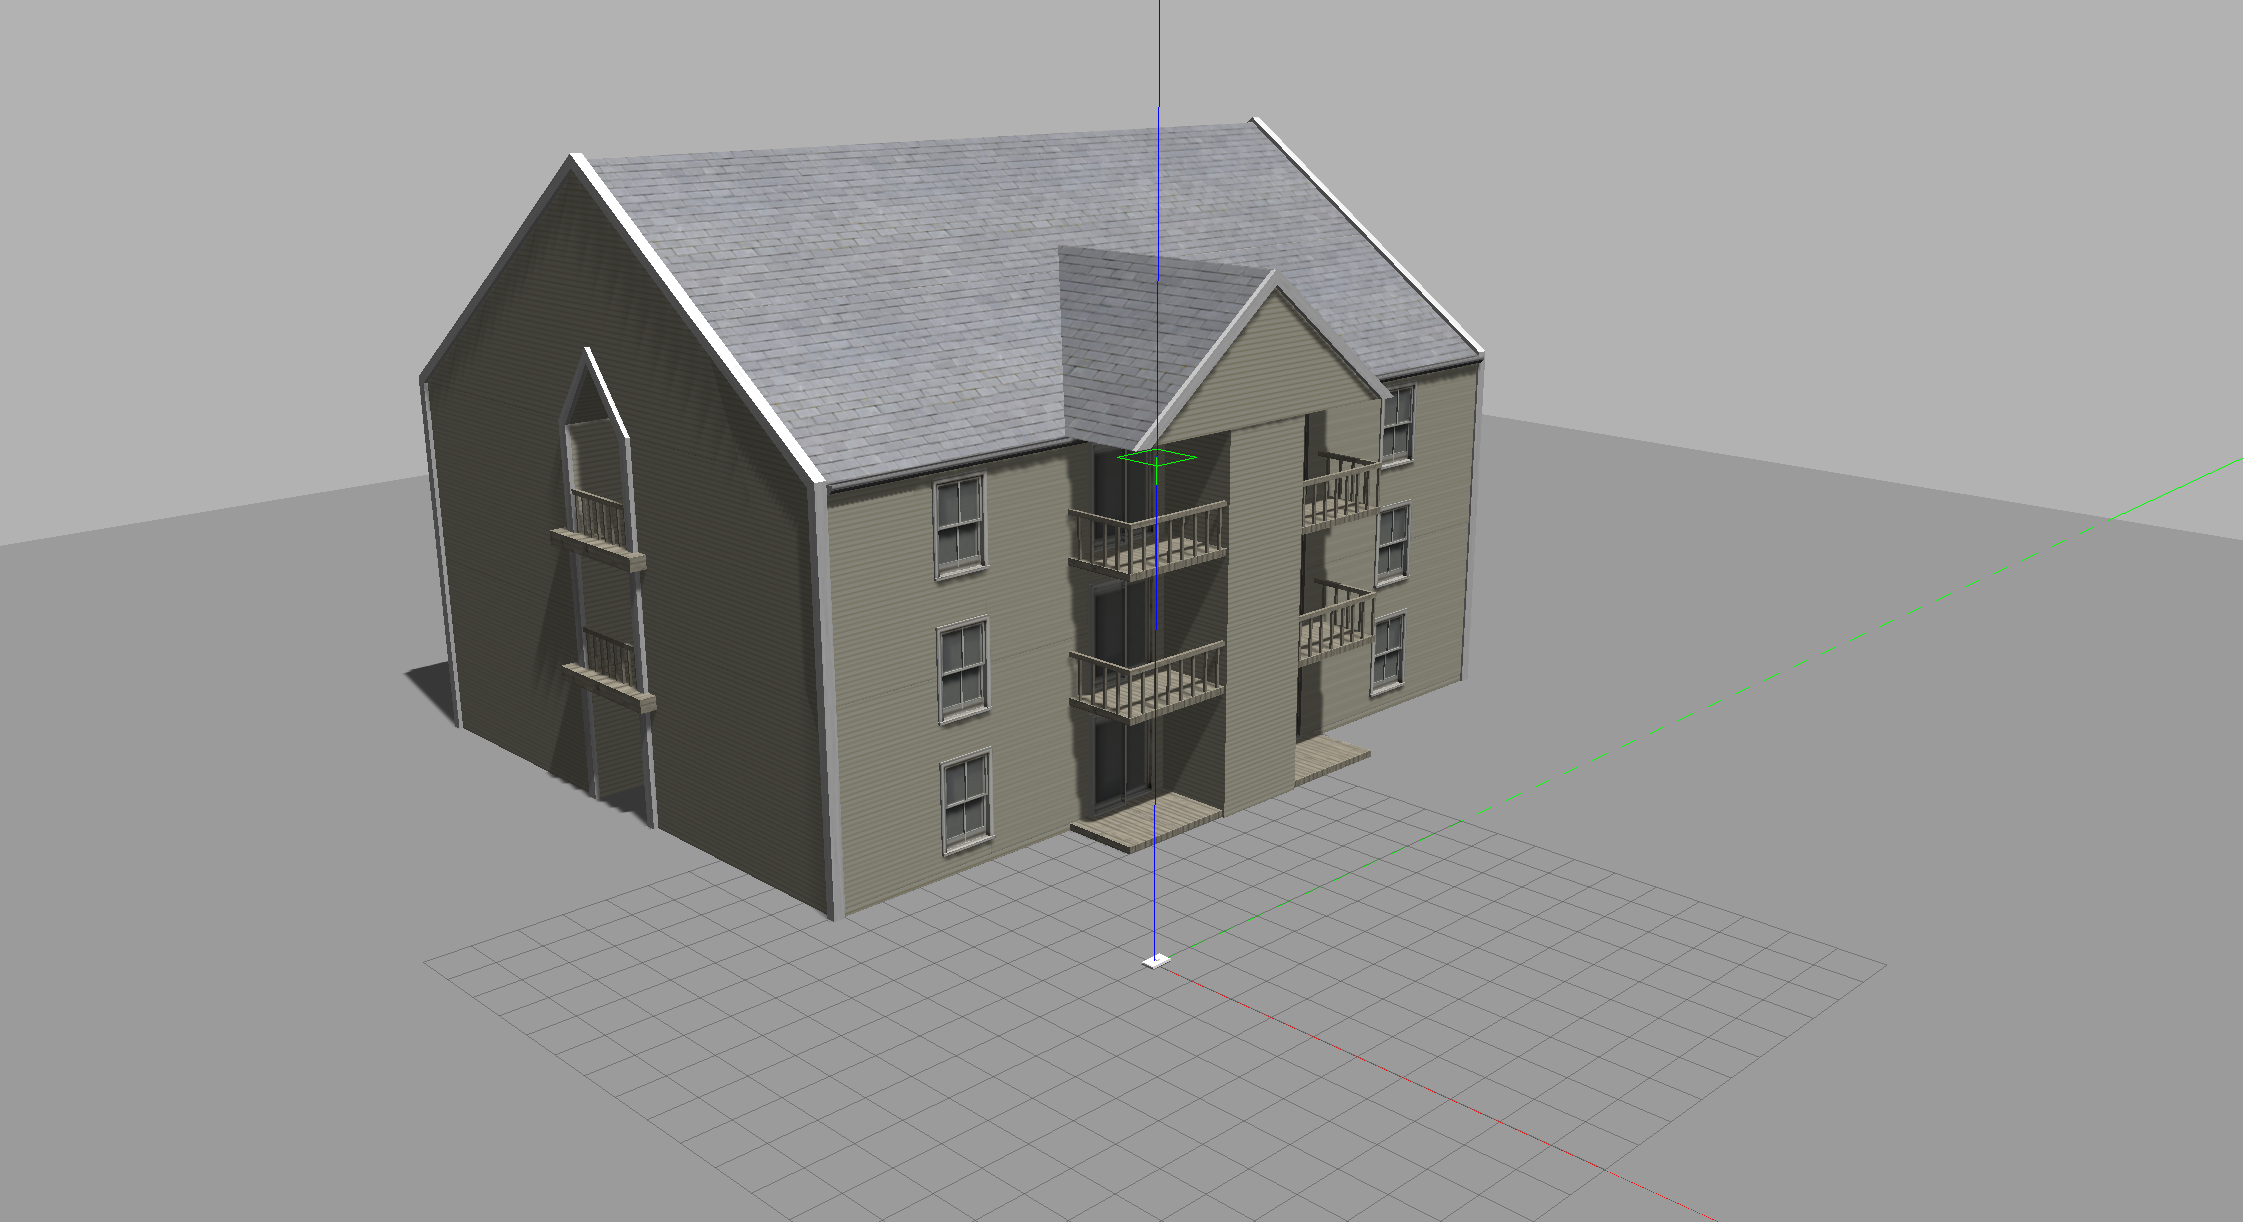
\includegraphics[height=0.25\textwidth]{Images/croped lidar simulation gazebo.png}}
                \subfigure[Point cloud from simulated lidar]{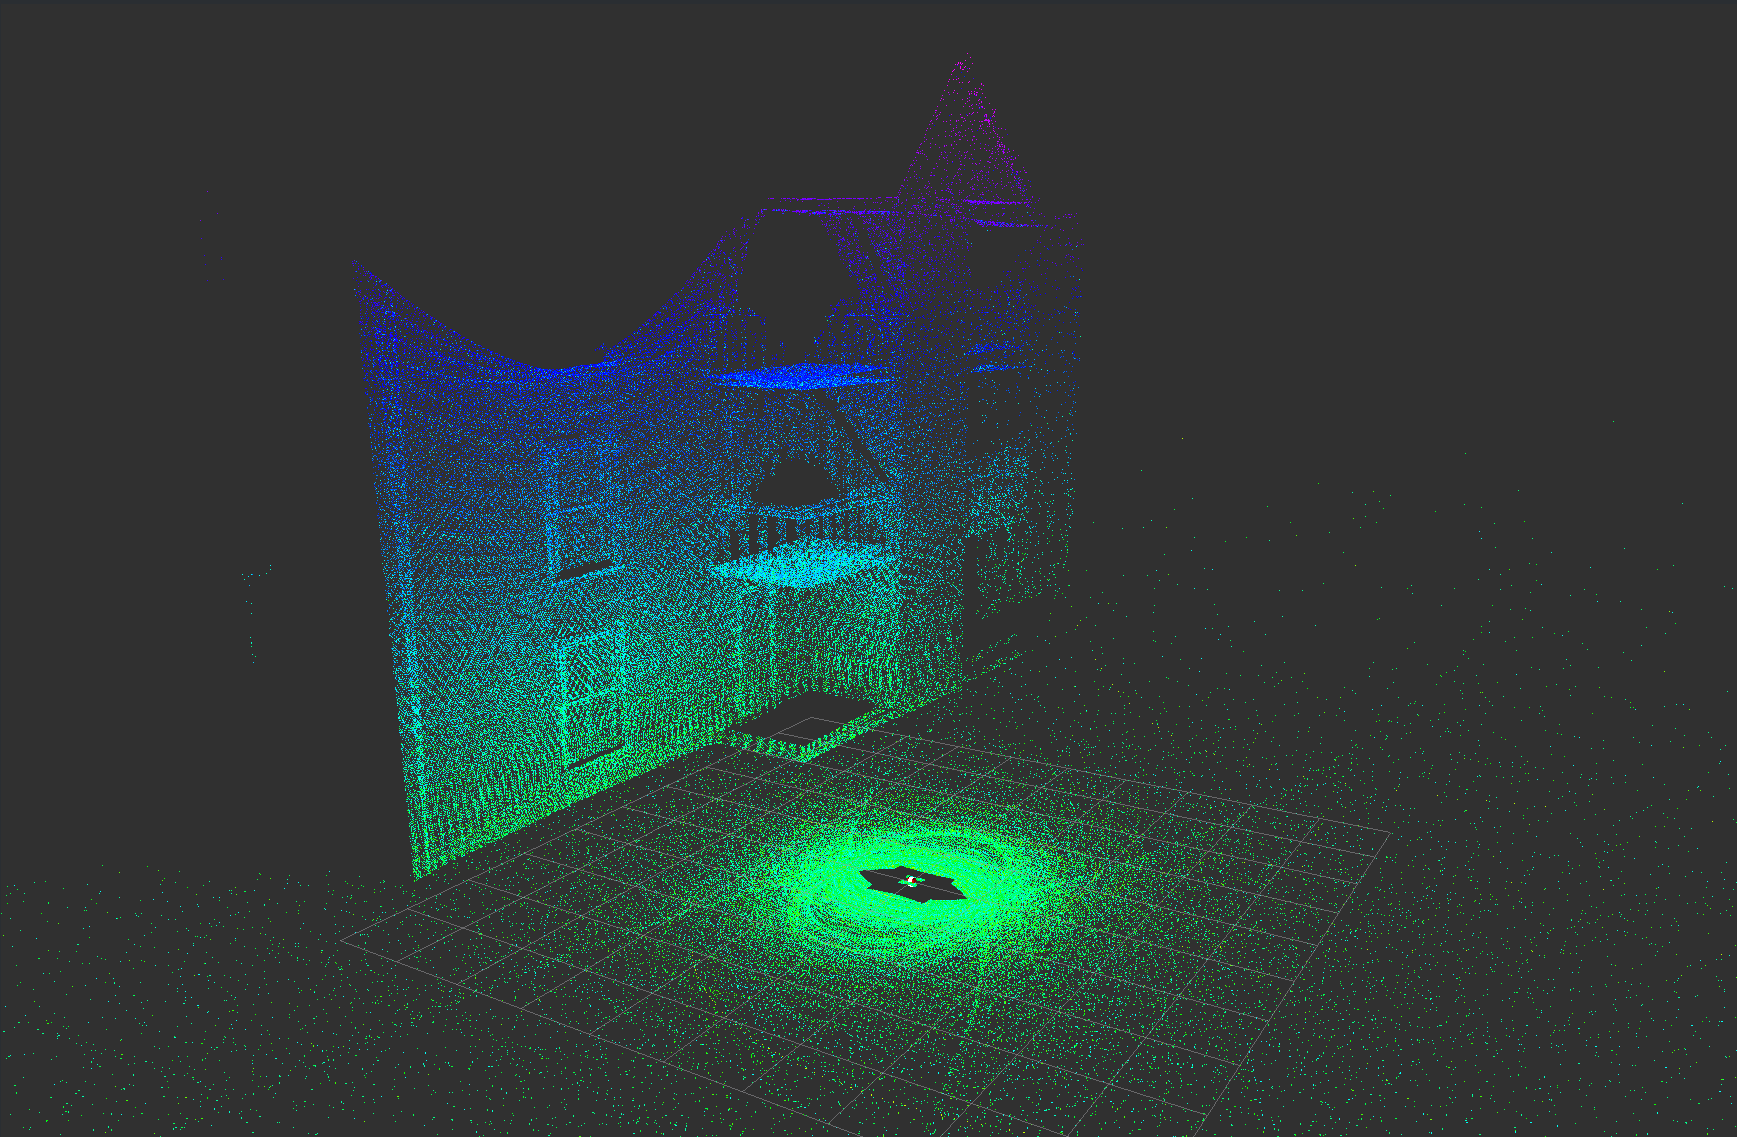
\includegraphics[height=0.25\textwidth]{Images/croped lidar simulation rviz2.png}}
                \caption{Simulated lidar in Gazebo and point cloud in RVIZ2}
            \end{figure}

            \subsubsection{IMU}
            \subsubsection{Camera}
        \subsubsection{Simulated world}


    \section{Conclusion}
    %\addcontentsline{toc}{section}{Conclusion}

        Conclusion     

    \newpage
    \bibliography{refs} % Entries are in the refs.bib file
    \addcontentsline{toc}{section}{Bibliography}

    \newpage
    \addcontentsline{toc}{section}{Glossaire}
    \printnoidxglossaries %glossaire, dans le fichier lexique.tex

    \newpage
    \addcontentsline{toc}{section}{List of figures}
    \listoffigures


    \newpage
    \section*{Annexe}
    \addcontentsline{toc}{section}{Annexe}
    Uncomment input annexe when needed
    %\begin{lstlisting}[style=yaml, caption={TARE planner parameter configuration for Unitree GO2}, label={lst:tare_config}]
tare_planner_node:
  ros__parameters:
    sub_start_exploration_topic_ : /start_exploration
    sub_terrain_map_topic_ : /terrain_map
    sub_terrain_map_ext_topic_ : /terrain_map_ext
    sub_state_estimation_topic_ : /state_estimation_at_scan
    sub_registered_scan_topic_ : /registered_scan
    sub_coverage_boundary_topic_ : /sensor_coverage_planner/coverage_boundary
    sub_viewpoint_boundary_topic_ : /navigation_boundary
    sub_nogo_boundary_topic_ : /sensor_coverage_planner/nogo_boundary
    sub_joystick_topic_ : /joy
    sub_reset_waypoint_topic_ : /reset_waypoint
    pub_exploration_finish_topic_ : exploration_finish
    pub_runtime_breakdown_topic_ : runtime_breakdown
    pub_runtime_topic_ : /runtime
    pub_waypoint_topic_ : /way_point
    pub_momentum_activation_count_topic_ : momentum_activation_count

    kAutoStart : true
    kRushHome : true
    kUseTerrainHeight : true
    kCheckTerrainCollision : true
    kExtendWayPoint : false
    kUseLineOfSightLookAheadPoint : false
    kNoExplorationReturnHome : false
    kExtendWayPointDistanceBig : 1.0
    kExtendWayPointDistanceSmall : 0.5  
    kKeyposeCloudDwzFilterLeafSize : 0.2
    kRushHomeDist : 0.05 # 5.0
    kAtHomeDistThreshold : 0.75 # 0.5
    kTerrainCollisionThreshold : 0.5
    kLookAheadDistance : 8.0
    kUseMomentum : false 
    kDirectionChangeCounterThr : 6
    kDirectionNoChangeCounterThr : 5
    kResetWaypointJoystickAxesID : 2

    # PlanningEnv
    kUseFrontier : true
    kFrontierClusterTolerance : 2.0 # 1.0
    kFrontierClusterMinSize : 5 #10
    kUseCoverageBoundaryOnFrontier : false
    kUseCoverageBoundaryOnObjectSurface : false

    # Rolling occupancy grid
    rolling_occupancy_grid/resolution_x : 0.2
    rolling_occupancy_grid/resolution_y : 0.2
    rolling_occupancy_grid/resolution_z : 0.2

    kSurfaceCloudDwzLeafSize : 0.3 # 0.3
    kCollisionCloudDwzLeafSize : 0.2 # 0.2
    kKeyposeCloudStackNum : 5 # 5
    kPointCloudRowNum : 20 # 50
    kPointCloudColNum : 20 # 50
    kPointCloudLevelNum : 30
    kMaxCellPointNum : 100000 # 100000
    kPointCloudCellSize : 5.0 # 18.0
    kPointCloudCellHeight : 1.8 # 1.8
    kPointCloudManagerNeighborCellNum : 5 # 5
    kCoverCloudZSqueezeRatio : 2.0 # 2.0

    # KeyposeGraph
    keypose_graph/kAddNodeMinDist : 1.0
    keypose_graph/kAddNonKeyposeNodeMinDist : 0.5
    keypose_graph/kAddEdgeConnectDistThr : 3.0
    keypose_graph/kAddEdgeToLastKeyposeDistThr : 3.0
    keypose_graph/kAddEdgeVerticalThreshold : 1.0
    keypose_graph/kAddEdgeCollisionCheckResolution : 0.4
    keypose_graph/kAddEdgeCollisionCheckRadius : 0.4
    keypose_graph/kAddEdgeCollisionCheckPointNumThr : 1

    # ViewPointManager
    viewpoint_manager/number_x : 30 # 50
    viewpoint_manager/number_y : 30 # 50
    viewpoint_manager/number_z : 1
    viewpoint_manager/resolution_x : 0.2 # 0.4
    viewpoint_manager/resolution_y : 0.2 # 0.4
    viewpoint_manager/resolution_z : 0.0
    kConnectivityHeightDiffThr : 0.25
    kGreedyViewPointSampleRange : 3 # 3
    kLocalPathOptimizationItrMax : 10 # 10
    kViewPointCollisionMargin : 0.25  # 0.6
    kViewPointCollisionMarginZPlus : 0.5
    kViewPointCollisionMarginZMinus : 0.5
    kCollisionGridZScale : 1.0
    kCollisionGridResolutionX : 0.2
    kCollisionGridResolutionY : 0.2
    kCollisionGridResolutionZ : 0.0
    kCollisionPointThr : 1
    kLineOfSightStopAtNearestObstacle : true
    kViewPointHeightFromTerrain : 0.3  # 0.75
    kViewPointHeightFromTerrainChangeThreshold : 0.2  # 0.6
    kCheckDynamicObstacleCollision : false
    kCollisionFrameCountMax : 3

    kSensorRange : 8.5  # 3.5
    kNeighborRange : 1.5 # 3.0
    kCoverageOcclusionThr : 0.1
    kCoverageDilationRadius : 0.9

    # Grid World
    kGridWorldXNum : 50 # 121
    kGridWorldYNum : 50 # 121
    kGridWorldZNum : 50 # 121
    kGridWorldCellHeight : 3.0 # 3.0
    kGridWorldNearbyGridNum : 5 # 5
    kMinAddPointNumSmall : 1 # 30
    kMinAddPointNumBig : 1 #60
    kMinAddFrontierPointNum : 1 #20
    kCellExploringToCoveredThr : 1
    kCellCoveredToExploringThr: 10 # 10
    kCellExploringToAlmostCoveredThr: 10 # 10
    kCellAlmostCoveredToExploringThr: 20 # 20
    kCellUnknownToExploringThr: 1

    # Visualization (parameters not working I think)
    kExploringSubspaceMarkerColorGradientAlpha : true
    kExploringSubspaceMarkerColorMaxAlpha : 0.8
    kExploringSubspaceMarkerColorR : 0.0
    kExploringSubspaceMarkerColorG : 1.0
    kExploringSubspaceMarkerColorB : 0.0
    kExploringSubspaceMarkerColorA : 1.0
    kLocalPlanningHorizonMarkerColorR : 0.0
    kLocalPlanningHorizonMarkerColorG : 1.0
    kLocalPlanningHorizonMarkerColorB : 0.0
    kLocalPlanningHorizonMarkerColorA : 1.0
    kLocalPlanningHorizonMarkerWidth : 0.05
    kLocalPlanningHorizonHeight : 3.0

\end{lstlisting}



    
\end{document}